% Lab 9, ALU with Input Register
% Created: 2020-04-2, Kyle Monk

%==========================================================
%=========== Document Setup  ==============================

% Formatting defined by class file
\documentclass[11pt]{article}

% ---- Document formatting ----
\usepackage[margin=1in]{geometry}	% Narrower margins
\usepackage{booktabs}				% Nice formatting of tables
\usepackage{graphicx}				% Ability to include graphics

%\setlength\parindent{0pt}	% Do not indent first line of paragraphs 
\usepackage[parfill]{parskip}		% Line space b/w paragraphs
%	parfill option prevents last line of pgrph from being fully justified

% Parskip package adds too much space around titles, fix with this
\RequirePackage{titlesec}
\titlespacing\section{0pt}{8pt plus 4pt minus 2pt}{3pt plus 2pt minus 2pt}
\titlespacing\subsection{0pt}{4pt plus 4pt minus 2pt}{-2pt plus 2pt minus 2pt}
\titlespacing\subsubsection{0pt}{2pt plus 4pt minus 2pt}{-6pt plus 2pt minus 2pt}

% ---- Hyperlinks ----
\usepackage[colorlinks=true,urlcolor=blue]{hyperref}	% For URL's. Automatically links internal references.

% ---- Code listings ----
\usepackage{listings} 					% Nice code layout and inclusion
\usepackage[usenames,dvipsnames]{xcolor}	% Colors (needs to be defined before using colors)

% Define custom colors for listings
\definecolor{listinggray}{gray}{0.98}		% Listings background color
\definecolor{rulegray}{gray}{0.7}			% Listings rule/frame color

% Style for Verilog
\lstdefinestyle{Verilog}{
	language=Verilog,					% Verilog
	backgroundcolor=\color{listinggray},	% light gray background
	rulecolor=\color{blue}, 			% blue frame lines
	frame=tb,							% lines above & below
	linewidth=\columnwidth, 			% set line width
	basicstyle=\small\ttfamily,	% basic font style that is used for the code	
	breaklines=true, 					% allow breaking across columns/pages
	tabsize=3,							% set tab size
	commentstyle=\color{gray},	% comments in italic 
	stringstyle=\upshape,				% strings are printed in normal font
	showspaces=false,					% don't underscore spaces
}

% How to use: \Verilog[listing_options]{file}
\newcommand{\Verilog}[2][]{%
	\lstinputlisting[style=Verilog,#1]{#2}
}




%======================================================
%=========== Body  ====================================
\begin{document}

\title{ELC 2137 Lab \#9: ALU with Input Register}
%%--------------------- EDIT HERE --------------------------
\author{Kyle Monk}
%%----------------------------------------------------------
\maketitle

\section*{Summary}
In this lab, an Arithmetic Logic Unit (ALU) was created that could do some simple calculations like addition and subtraction, as well as combinational logic like AND, OR, and XOR. One of the numbers being operated on was inputted through the switches in a basys3 board, while a register was used to store a second number. 

\section*{Expected results tables}

\begin{table*}[ht]\centering
	\caption{\textit{register} expected results table}
	\label{ALU:tbl:register_ERT}\medskip
	\begin{tabular}{l|rrrrrrrrrrr}
		Time (ns): & 0-5 & 5-10 & 10-15 & 15-20 & 20-25 & 25-30 & 30-35 & 35-40 & 40-45 & 45-50 & 50-55 \\
		\midrule
		D (hex) & 0 & 0 	  & A & A & 3 	    & 3 	  & 0 	    & 0 & 0$\to$6 & 6 & 6 \\
		clk     & 0 & 1 	  & 0 & 1 & 0 	    & 1 	  & 0 	    & 1 & 0 	  & 1 & 0 \\
		en  	& 0 & 0 	  & 1 & 1 & 1$\to$0 & 0$\to$1 & 1$\to$0 & 0 & 0$\to$1 & 1 & 1 \\
		rst 	& 0 & 0$\to$1 & 0 & 0 & 0 		& 0 	  & 0		& 0 & 0		  & 0 & 0 \\
		\midrule
		Q (hex) & X & X$\to$0 & 0 & A & A & A & A & A & A & 6 & 6 \\
		\bottomrule
	\end{tabular}
\end{table*}

\begin{table*}[ht]\centering
	\caption{\textit{alu} expected results table}
	\label{ALU:tbl:alu_ERT}\medskip
	\begin{tabular}{l|rrrrrr}
		Time (ns): & 0-10 & 10-20 & 20-30 & 30-40 & 40-50 & 50-60 \\
		\midrule
		in0 & 14 & 14 & 14 & 14 & 14 & 14 \\
		in1 & 7A & 7A & 7A & 7A & 7A & 7A \\
		op	& 0 & 1 & 2 & 3 & 4 & 5 \\
		\midrule
		out & 8E & 9A & 10 & 7E & 6E & 14 \\
		\bottomrule
	\end{tabular}
\end{table*}

\section*{Results}

\begin{figure}
	\centering
	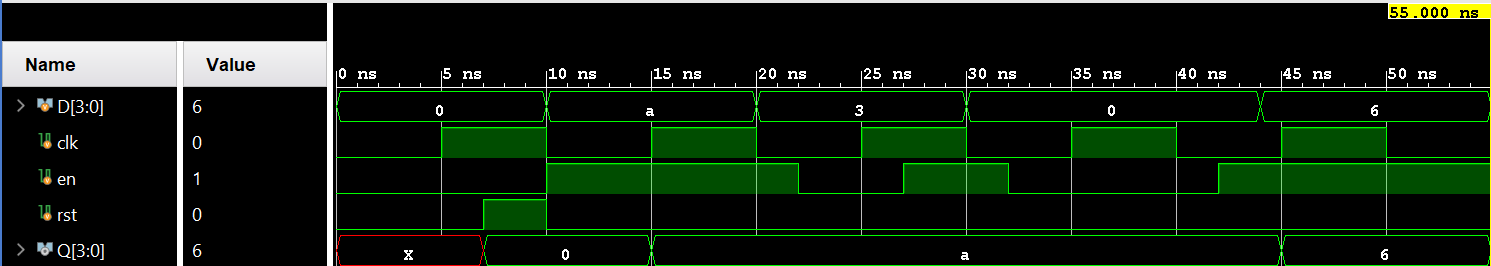
\includegraphics[width=1\linewidth]{register_test}
	\caption{Register Simulation Waveform}
	\label{fig:registertest}
\end{figure}

\begin{figure}
	\centering
	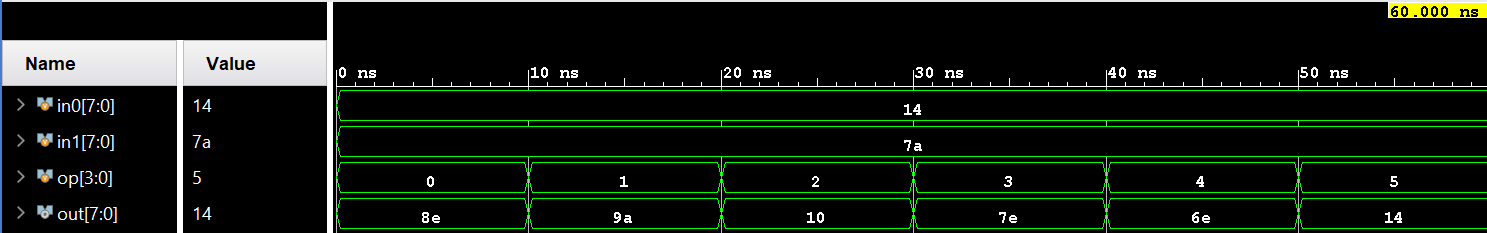
\includegraphics[width=1\linewidth]{alu_test_CORRECTED}
	\caption{ALU Simulation Waveform}
	\label{fig:alutest}
\end{figure}



\begin{figure}
	\centering
	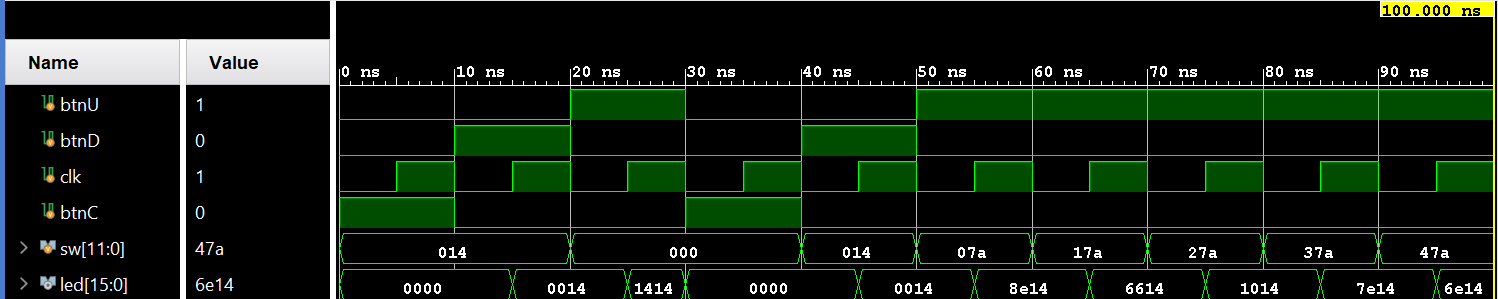
\includegraphics[width=1\linewidth]{basys3_lab9}
	\caption{Top Level Simulation Waveform}
	\label{fig:basys3lab9}
\end{figure}

\clearpage

\section*{Code}
\begin{lstlisting}[style=Verilog,
caption=register Design,
label=code:ex1]
`timescale 1ns / 1ps
//Lab 9, Created by Kyle Monk 04-01-20

module register #( parameter N =1)
(
input clk , rst , en ,
input [N -1:0] D ,
output reg [N -1:0] Q
) ;
always @ ( posedge clk , posedge rst )
begin
if ( rst ==1)
Q <= 0 ;
else if ( en ==1)
Q <= D ;
end

endmodule

\end{lstlisting}

\begin{lstlisting}[style=Verilog,
caption=register\_test Design,
label=code:ex2]
`timescale 1ns / 1ps
//Lab 9, created by Kyle Monk 04-01-20

module register_test () ;
reg [3:0] D ;
reg clk , en , rst ;
wire [3:0] Q ;
register #(. N (4) ) r (. D ( D ) , . clk ( clk ) ,
. en ( en ) , . rst ( rst ) , . Q ( Q ) ) ;
// clock runs continuously
always begin
clk = ~ clk ; #5;
end
// this block only runs once
initial begin
clk =0; en =0; rst =0; D =4'h0 ; #7;
rst = 1; #3; // reset
D = 4'hA ; en = 1; rst = 0; #10;
D = 4'h3 ; #2;
en = 0; #5;
en = 1; #3;
D = 4'h0 ; #2;
en = 0; #10;
en = 1; #2;
D = 4'h6 ; #11;
$finish ;
end
endmodule
\end{lstlisting}

\begin{lstlisting}[style=Verilog,
caption=ALU Design,
label=code:ex3]
`timescale 1ns / 1ps
//Lab 9, created by Kyle Monk 04-01-20

module alu #( parameter N =8)
(
output reg [N -1:0] out ,
input [N -1:0] in0 ,
input [N -1:0] in1 ,
input [3:0] op
) ;
// Local parameters
parameter ADD =0;
parameter SUB =1;
parameter AND =2;
parameter OR =3;
parameter XOR =4;
always @ *
begin
case ( op )
ADD : out = in0 + in1 ;
SUB : out = in0 - in1;
AND : out = in0 & in1;
OR : out = in0 | in1;
XOR : out = in0 ^ in1;
default : out = in0 ;
endcase
end
endmodule
\end{lstlisting}

\begin{lstlisting}[style=Verilog,
caption=ALU\_test Design,
label=code:ex4]
`timescale 1ns / 1ps
//Lab 9, created by Kyle Monk, 04-01-20

module alu_test();

reg [7:0] in0, in1;
reg [3:0] op;
wire [7:0] out;

alu #(.N(8)) a(.in0(in0), .in1(in1), .op(op), .out(out));
initial begin
op = 0; in0 = 8'h14; in1 = 8'h7A; #10;
op = 1; in0 = 8'h14; in1 = 8'h7A; #10;
op = 2; in0 = 8'h14; in1 = 8'h7A; #10;
op = 3; in0 = 8'h14; in1 = 8'h7A; #10;
op = 4; in0 = 8'h14; in1 = 8'h7A; #10;
op = 5; in0 = 8'h14; in1 = 8'h7A; #10;
$finish;
end
endmodule
\end{lstlisting}

\clearpage

\begin{lstlisting}[style=Verilog,
caption=top\_lab9 Design,
label=code:ex5]
`timescale 1ns / 1ps
//Lab 9, created by Kyle Monk 04-01-20

module top_lab9(
input btnU, btnD, clk, btnC, input [15:0] sw, 
output [15:0] led);

wire [7:0] r1out, aluout, r2out;

register #(.N(8)) r1(.clk(clk), .D(sw[7:0]), .en(btnD), .rst(btnC), .Q(r1out));
alu #(.N(8)) a1(.in0(sw[7:0]), .in1(r1out), .op(sw[11:8]), .out(aluout));
register #(.N(8)) r2(.clk(clk), .D(aluout), .en(btnU), .rst(btnC), .Q(r2out));
assign led = {r2out, r1out};

endmodule
\end{lstlisting}

\end{document}
